\documentclass{tufte-handout}
\usepackage{amsmath,amsthm}
\usepackage{bm}


\input{vc.tex}

\usepackage{pgfplots}
\pgfplotsset{width=\textwidth,compat=1.5.1}

\newtheorem{claim}{Claim}[section]
\title{\sf Markov Chains and Random Processes}
\date{\GITAuthorDate}
\author{M\aa ns Magnusson}

\begin{document}
\maketitle
\footnotetext{rev. \GITAbrHash}

\emph{2017 is the first year this lab is given. Some errors in the instructions are expected.}

\section{FedUPS vs PostNHL}

You are having a hard time choosing between the two major post companies in your city.

\medskip

They have the same price, they have negligible customer service, 
and their delivery strategy is exactly the same, except that they start from different warehouses.

The strategy is the following: a driver starts from a warehouse which lays in direct connection to an intersection. 
Whenever a driver arrives at an intersection $I$ a road to the next intersection is picked at random, given some fixed probability distribution for roads going out from $I$. 
Each intersection is connected with roads to at least one other intersection. It takes a fixed time to drive along each road. 
If a driver arrives to the intersection you live by the driver delivers your package. (You never leave your house).

\medskip

You'd like to pick the post company that has the lowest estimated delivery time.


\section*{Input}
The first line contains 5 integers, $N\, M\, H\, F\, P$, where $3 \leq N \leq 300$ is the number of intersections, 
$\frac{N}{2} \leq M \leq \frac{N(N-1)}{2}$ is the number of roads, $0 \leq H < N$ is the intersection id you live by, and 
$0 \leq F\, P < N$ are the intersection ids for FedUps and PostNHL respectively. 

\medskip

Then follow $M$ lines describing each road.

\medskip

A road is descibed by 5 numbers, $u\, v\, t_{uv}\, p_{uv} \, p_{vu}$ where $u$ and $v$ are the ids of the intersections the road connects, 
$t_{uv}$ is an integer describing the time in minutes it takes to travel along the road. 
$p_{uv}$ describes the probability of choosing to travel from $u$ to $v$ if you are at intersection $u$, 
while $p_{vu}$ is the probability of traveling from $v$ to $u$ if you are located at intersection $v$.

\medskip

All probablities $p_{uv}$ where $u \neq H$ satisfy $0 < p_{uv} \leq 1$.

It is guarnteed that for each intersection the total probability of leaving that city is $1.0$,
except for the the intersection $H$, where the driver stops and delivers your package, 
hence here the probablity of leaving is $0$.

\section*{Output}
Output the estimated delivery time in minutes for each post company.
If your home is not reachable by a delivery company, output ``We tried to deliver your package, but you were not at home''.


\section*{Algorithm Monte-Carlo}
We can simulate the drivers traversing the graph until they reach your home.
Taking the average of this algorithm will converge towards the estimated delivery time.
The simulation picks a random road according to the probability distrubution 
of the node the driver is at until the driver reaches your home. While doing this we accumelate the time.
\begin{marginfigure}
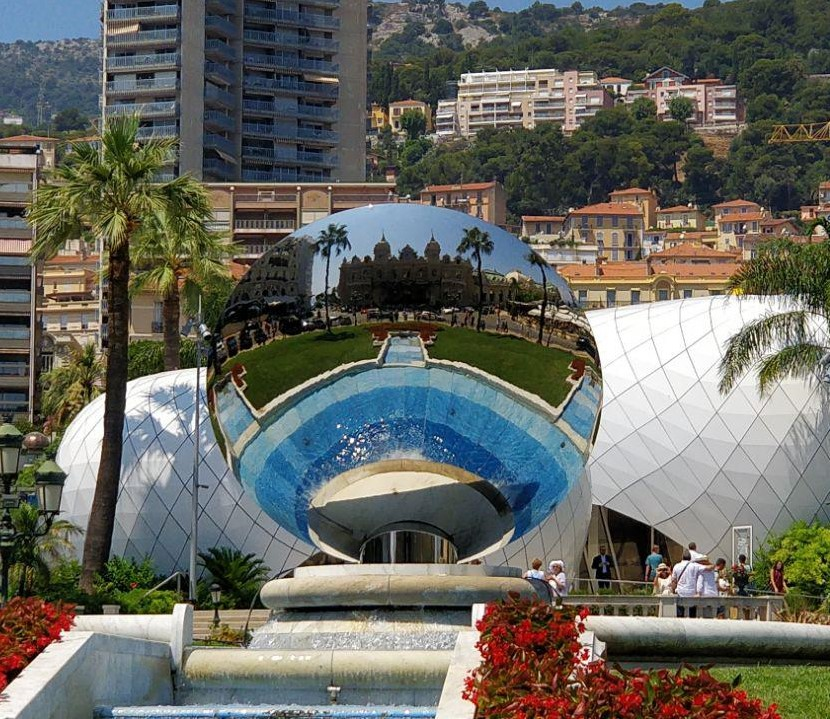
\includegraphics[width=2in]{montecarlo.jpg}
\caption{\emph{The casino in Monte Carlo} Photographer: Maj Stenmark (2017). Licence: Creative Commons Attribution-ShareAlike}
\end{marginfigure}


\section*{Algorithm Markov}
We can view this problem as a markov chain. 
Let $x_u$ denote the estimated time left until the driver reaches node $H$ from node $u$.
$x_u$ can be expressed as a sum over all it's neighbours.

$x_u = \sum_{uv \in E}{p_{uv}\cdot (x_v + t_{uv})}$

This can be written as a system of equations

$\bm{x} = \bm{Ax} + \bm{b}$
where $\bm{A}$ is a matrix, and $\bm{A}_{u,v} = p_{uv}$. $\bm{b}$ is a vector, and $\bm{b}_u = \sum_{uv \in E}{p_{uv}\cdot t_{uv}}$

We then get $(\bm{A}-\bm{I})\bm{x} = -\bm{b}$, which can be solved with gaussian elimination.

We then have the estimated delivery time for each node.

\subsection{Deliverables}

\begin{enumerate}
\item Implement the Monte-Carlo and Markov algorithms.
\item Run them on all the test cases in the data directory.
\item You can use Octave to solve the system of equations for you, 
    however we expect you to run the code on all of the testcases with a script.
    Other options include using numpy, or implement/finding an implementation of
        Gaussian Elimination in the language you are using.\sidenote{Remember that it`s easy to verify the solution of Guassian elimination. 
        Do this if you encounter problems with your Markov implementation.}
\item Fill out the report on the next page; you can just use the
  \LaTeX\ code if you want.
\end{enumerate}

\newpage


\newpage
\section{FedUPS Lab Report}


by Alice Cooper and Bob Marley\sidenote{Complete the report by filling
  in your names and the parts marked $[\ldots]$.
  Remove the sidenotes in your final hand-in.}


\subsection{Solution quality Toy}

Running the Monte-Carlo algorithm $10\,000$ runs takes $[\ldots]$ seconds to execute, before reaching an accuracy within $[\ldots]$ digits
\sidenote{Here we are after the relative accuracy, which we define as the number of leading zeroes in the expression $\frac{E[G] - Avg(MonteCarlo(G))}{E[G]}$, where $E[G]$ is the estimated delivery time.} 
of accuracy on the input toy.in.\sidenote{Take the minimum of FedUPS and PostNHL compared to the output file.}


\subsection{Solution quality Small}

$[\ldots]$ runs, and $[\ldots]$ seconds are needed for the Monte-Carlo algorithm on input small.in to be within $3$ digits of accuracy for 10 consecutive runs.\sidenote{
    You should compare the accuracy versus the result of your Markov Algorithm, which solves the problem exactly. Both FedUPS and PostNHL needs to be stable.
}

\subsection{Results of the Markov Algorithm}

\begin{tabular}{c c c}
    input graph & $E[\text{FedUPS}]$ & $E[\text{PostNHL}]$ \\
    random1.in & $[\ldots]$ & $[\ldots]$ \\
    random2.in & $[\ldots]$ & $[\ldots]$ \\
    random3.in & $[\ldots]$ & $[\ldots]$ \\
    strange1.in & $[\ldots]$ & $[\ldots]$ \\
    strange2.in & $[\ldots]$ & $[\ldots]$ \\
\end{tabular}\sidenote{If you encounter problems with strange1.in or strange2.in draw the graphs. Remember what you did to solve them for the next sections.}

\subsection{Stranger Things}
$[\ldots]$ happens when the original versions of the algoritms were run on the graph strange1.in. 
This is because node $F$ and $P$ are $[\ldots]$ from node $H$. We fixed this by ${\ldots}$.

\subsection{Stranger Things 2 - Pre Realease}
Out of the original versions of the algorithms, only algorithm $[\ldots]$ works on the graph strange2.in. 
The reason algorithm $[\ldots]$ does not work is that the graph is $[\ldots]$, which results in $[\ldots]$.


\subsection{Real real world problems}
The problem FedUPS vs PostNHL is a very constructed problem. 
This is used as an exercise in identifying that a problem can be modeled as a Markov Chain.
However in the real world examples of problems that include markov chains include $[\ldots]$ and $[\ldots]$.

\end{document}
